%!TEX root = ../thesis.tex
%*******************************************************************************
%****************************** Second Chapter *********************************
%*******************************************************************************
\chapter{The LHC and CMS}

\section{The Large Hadron Collider}
\begin{linenumbers}
The Large Hadron Collider (LHC) is one the  largest and most powerful particle accelerator in the world. It came on operation on 10 September 2008 and it is the most recent addition from the  European Organization for Nuclear Research (CERN).  The LHC is a 27 kilometer ring composed of  superconducting magnets with accelerating structures to boost the energy of the particles. \\

The LHC is designed to accelerate particles to high energies and generate collisions. There are several
experiments installed along the LHC ring. One of them is ATLAS, located on Point 1 between the two injection lines , which is a general purpose detector. From ATLAS at point 5 is another general purpose detector,the compact muon solenoid  (CMS). A particle detector optimized for heavy ion physics, ALICE, is located at Point 2 and LHCb, a detector designed for B physics, is located at Point 7.\cite{cern1,cern2}
\\

Inside the accelerator, two high energy particles beams travel at
close to the speed of light before they collide. 
In order to make them collide, beams travel in opposite directions in separate beam pipes, 
two tubes kept at ultrahigh vacuum. 
By using of superconducting electromagnets that generates a powerful magnetic field , the beams are guided around the accelerator ring. \\
The electromagnets are built from coils of special electric cable that operates in a superconducting state, efficiently conducting electricity without resistance or loss of energy.For that, it is required to have  magnets to a temperature of  $‑271.3$ C. 
For reach such temperatures, a system of liquid helium is connected to the accelerator.\cite{cern2}

\pagebreak

\begin{figure}[!htbp]
\centering
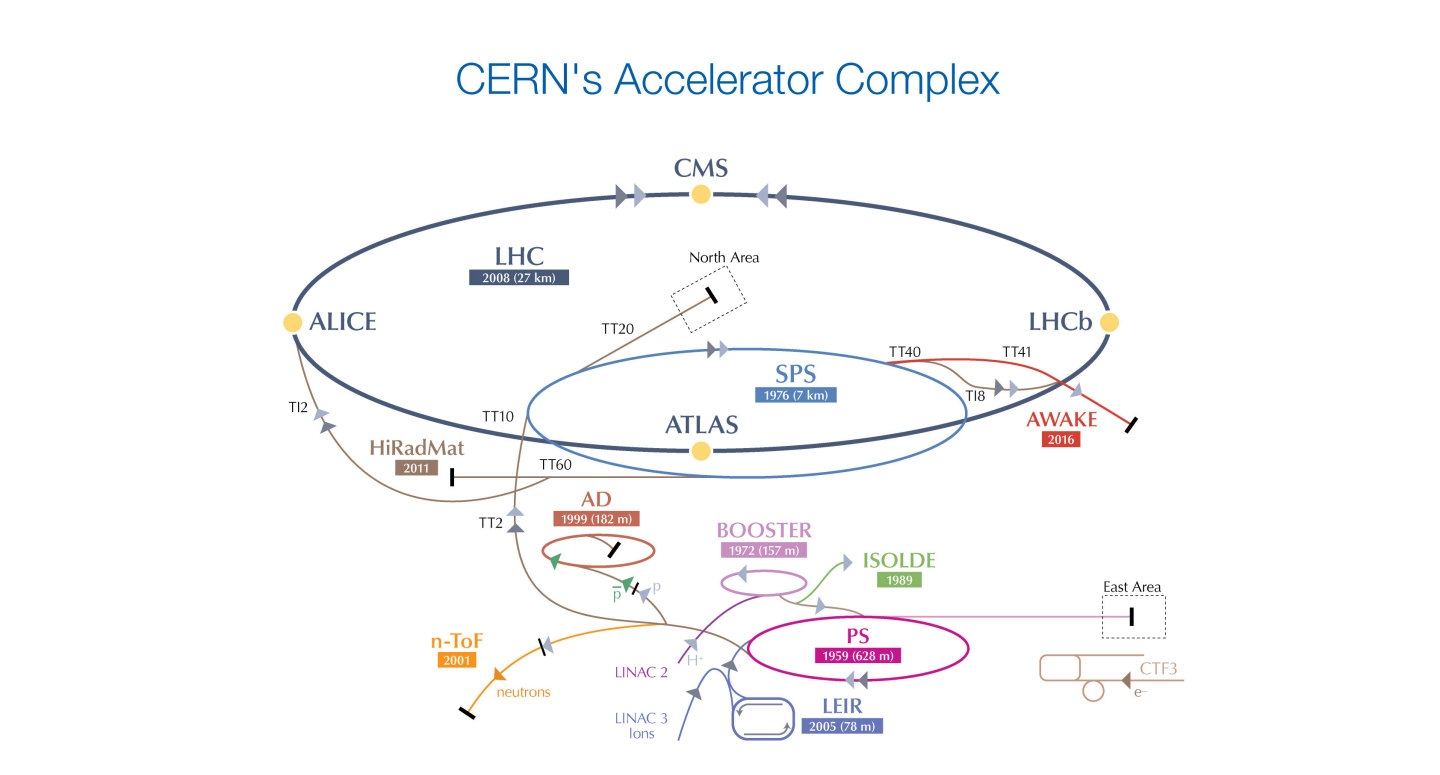
\includegraphics[width=17cm,height=11cm]{Chapter1/cern.jpg}
\caption{Large hadron collider from CERN} \label{lhc}
\end{figure}


The process for the beam collision comes on various stages inside of the collider, which also is composed of smaller particle accelerators.\\
Protons in the LHC start out as hydrogen atoms stripped of their electrons. The first accelerating stage the protons are subjected to is a linear accelerator, Linac2,
which accelerates them up to 50 MeV . The protons are then sent into the
Proton Synchotron Booster which accelerates them up to 1.4 GeV before sending them to the Proton Synchotron (PS). The protons leave the PS at 25 GeV before entering the Super Proton Synchotron (SPS), which accelerates them to the LHC injection energy of 450 GeV. After this stage, the beam is ready to be injected into
the LHC through one of two injection lines with 6.5 TeV.\cite{cern3}

\begin{table}[!htbp]
\centering
	\caption{Accelerator operation energies}
	\begin{tabular}{|c|c|}
		\hline
		Accelerator & Energy \\
		\hline
		Linac 2 &  50 MeV \\
		\hline
		PS Booster & 1.4 GeV \\
		\hline
		Proton Scyncroton (PS) & 25 GeV\\
		\hline
		SPS &  450 GeV\\
		\hline
		LHC & 6.5 TeV\\
		\hline
	\end{tabular}
\end{table}
\pagebreak
Inside the accelerator, collided protons generates an amount of particles such as pion and kaons, which are the most commons, created by the jet particles that were created after the collision. Besides of the particles created by the quarks of the proton shattered, gluons are also radiated and create new particles and photons are radiated too. \\
During the collision time, the main  detectors of LHC capture the energy signal
and save the data in supercomputers. Those high end computers starts to measure the energy signals in order to asign a type of events.
\\

The main objetive of the LHC is to study the nature of electroweak symmetry breaking for the Higgs mechanism is associated. 
The experimental study of the
Higgs mechanism can also  verify the mathematical results  the Standard Model at higher energy scales.\\
Alternatives to the Standard Model that involves different symmetries are also put on test. With the exploration of theses theories, people have hope for a discovery that guide them toward a unified theory, so the importance to accelerate particles to higher energy scales.
\\
For improve the results of experiments, the LHC has a schedule where there is a period of experiments that last for three years. Ending the experimental time, the engineers of the LHC start the maintenance time which last between three or four years.  

\begin{figure}[!htbp]
\centering
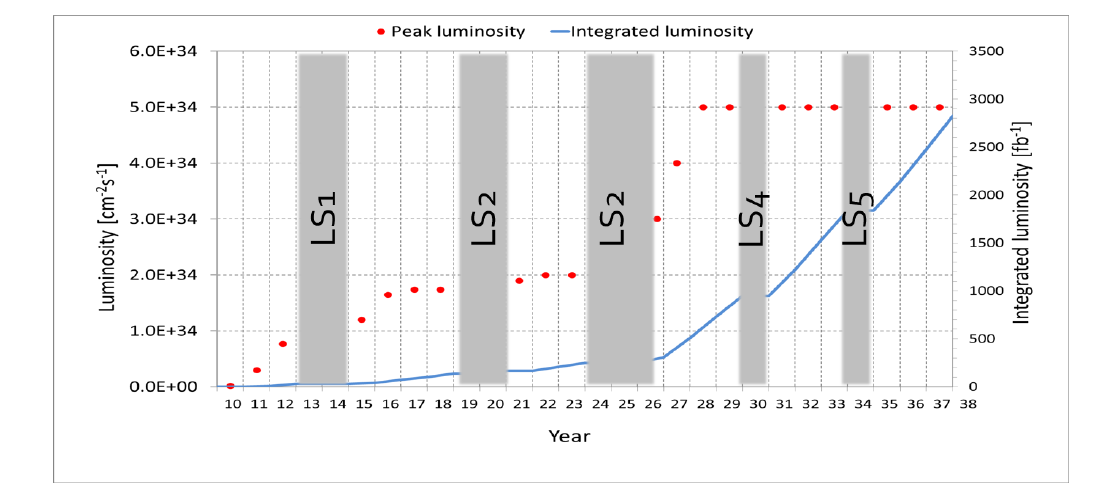
\includegraphics[scale=0.5]{Chapter2/lum6.png}
\caption{LHC schedule, including future plans for increase the center of mass energy and luminosity. %
\cite{cern3}}
\label{lhc-lumi}
\end{figure}
From the figure \ref{lhc-lumi}, shows the Large Hadron Collider forecast for the increase of luminosity for the next years. Red dots are peak luminosity expected to reach and blue line is integrated luminosity.  \\
In the year 2018, the maximum integrated luminosity is around 150 $fb^{-10}$\cite{cern3}. From 2019 to 2021 the second phase of maintenance, where engineers increase the performance of the accelerator, give maintenance to the system and introduce new components to the complex. After that period, the LHC starts new collision experiments at even higher energies in order to explore new particle phenomena.


\pagebreak

\section{The Compact Muon Solenoid}	
The Compact Muon Solenoid (CMS) is a detector with multiple uses in the LHC and part of the main experiments at CERN. Located underground in the France Switzerland border , in the city of Cessy, France.
This detector was designed in the early 1990s, based on the mass limit of the Higgs boson,  and put on operation in 2008,  it is a big solenoid of  that generates a great magnetic field of 4 teslas with the objective to separate particles after a particle collision.
 The detector has 21 metres long, 15 metres wide and 15 metres high.
Inside of the complex, there are many layers of detectors to register different kinds of energy signals. But since muons go through materials very easy, the complex is buried 100 meters underground.\\ 

The CMS experiment is composed of several detector layers called chambers that allow identify and save different types of energy signals (momentum) and it is saved in a powerful supercomputers that separate and classify the data according to certains variables. The general parts of the CMS are the Silicon tracker , an electromagnetic calorimeter,a hadron calorimeter, the solenoid (superconducting magnet) and the muon detector layer. \\

The magnet is a big superconducting solenoid that generates a magnetic field of 4 Teslas. The magnet is 13 m long and it has a diameter of 5.9 m with a weight of 12000 ton. The reason for such a strong magnetic field is for obtain a better momentum resolution combined with the alignment of the detectors.
The magnetic flux is returned via a 1.5 m thick saturated iron yoke instrumented with four stations of muon
chambers.

\begin{table}[ht]
	\caption{Characteristic of the CMS superconducting solenoid \cite{cms-manual}}
	\centering
	\begin{tabular}{|c|c|}
		\hline
		Field strength & 4 T \\
		Inner Bore & 5.9 m \\
		Length & 12.9 m\\
		Number of Turns & 2168\\
		Current & 19.5 kA\\
		Stored energy & 2.7 GJ\\
		Hoop stress & 64 atm\\
		\hline
	\end{tabular}
	\label{tab:my_label}
\end{table}






%The trigger or event selection process must reduce the approximately 1 billion interactions per second to more less than 100 events per second for storage and subsequent analysis.\\

 The objetives of the CMS experiment are numerous. One of them is
identification of muons by measuring the momenta and scattering angle. Search for evidence  and give proof of super symmetry  for show evidence of BSM (Beyond Standard Model). Detection of massive vector bosons $W^\pm$ and Z via $e^+e^-$ and $\mu^+ \mu^-$ decays.\\
Search for extra dimensions from BSM theory that could be related to production of particles and quantum gravity. Study of QCD, electroweak and flavor physics to detect new decays predicted by SM at higher energies. Heavy ions collision experiments for the study of production of  very strongly interacting nuclear matter\cite{cms-manual}.
This experiment along the ATLAS experiment discovered the Higgs boson in 2012.
\\


\subsection{Silicon Tracker}



\subsection{Electromagnetic calorimeter}

The electromagnetic calorimeter or ECAL is a calorimeter composed of 61200 lead tungstate (PbWO$_4$) crystals that act as scintillanting crystals (emits light when particles interact with the crystal). These calorimeters are mounted in the central barrel and closed by 7324 crystals in the both endcaps. The barrel section  of the ECAL covers the pseudorapidity range $|\eta| < 1.479$. The crystals in the barrel have a pyramid shape and their crosss section is 22$\times$22 mm$^2$ at the front face and 26$\times$26 mm$^2$ at rear face. The crystal length is 230 mm.  The crystals are stored in a thin walled glass-fibre alveola structures that have the same shape. These structures are assembled in modules  and arranged in arrays of four separated by aluminium webs.The EB (barrel section of ECAL) has a inner radius of 129 cm\cite{cms-manual}\\

The endcaps cover have the  range 1.479 < $|\eta|$ < 3.0. The distance between the interaction point and the endcap is 3.144 m. The endcap has  identically shaped crystals grouped in
mechanical units of 5×5 crystals (supercrystals, or SCs) consisting of a carbon-fibre alveola
structure. The crystal cross section for the rear face is 30 $\times$ 30 mm$^2$ , 28.62 $\times$ 28.62 mm$^2$ and a length of 220 mm.
\\

In the barrel, there photodetectors called avalanche photodiodes (APD), made of silicon with a active area of  5 $\times$ 5 mm$^2$ with 2 glued to the back of each crystal. These have a operating voltage of 5 V and paired they reach a voltage between 340 to 430 V. At the endcap , the photodetectors are vacum photodiodes (VPT) that are photomultipliers having a single gain stage , made of with an anode of copper mesh (10 $\mu m$) , allowing to operate in the magnetic field. VPT have a size of 25 mm in diameter , glued to the back of each crystal.\\

There is also a preshower detector , which principal function  is to identify neutral pions in the
endcaps within the region 1.653 < |$\eta$| < 2.6. It also helps the identification of electrons
against minimum ionizing particles, and improves the position determination of electrons and photons.  %The ES is a sampling calorimeter with 2 layers: lead
%radiators initiate electromagnetic showers from incoming photons/electrons whilst silicon
%strip sensors placed after each radiator measure the energy deposited and the transverse shower profiles.


\subsection{Hadron calorimeter}
The hadron calorimeter (HCAL) along the ECAL, form a complete calorimeter that allows to measure the jets and missing transverse energy. HCAL is located in the barrel and the endcaps, surrounding the ECAL and affected by the magnetic field generated by the solenoid.\\
The Barrel section (HB) and endcap section (HE)  cover the pseudorapity 0 < $|\eta|$ < 1.3 and  1.3 < $|\eta|$ < 3.0 respectively.\\
The HB is an assembly of two half barrels, composed of 18 parts of brass alloy plates in wedge shape. These absorber plates in the innermost and outermost are made of stainless steel and brass respectively.\\
The longitudinal profile in the barrel going from an inner radius of 1777 mm to an outer radius of 2876.5 mm, divided by 17 plastic scintillador between the brass and stainless plates. Each scintillator are instrumented with a single wave 
lenght shifting fibers (WLS). Those fibers allows to carry the light from the scintillator to the readout system.\\


There is also a foward calorimeter (HF) located at 11.2 m from the interaction point, that cover the region of 2.9 < $|\eta|$ < 5, designed to measure the energy of foward jets but optimized for 



\subsection{Muon detector}
 The muon detector system in the Compact Muon Solenoid (CMS) experiment  has 3 primary functions: muon
triggering, identification, and momentum measurement\cite{cms7}. 
The process utilized in the CMS muon chamber systems is gas ionization. Those gas-ionization particle detectors are arranged in a cylindrical barrel region and planar endcaps, in order to meet the geometry of the solenoid.The barrel detector is built with 4 station of 250 chambers inside the magnet return yoke.\cite{cms-manual}
 There are three main detectors used in the muon chamber: the drift tubes chambers (DT), the cathode strips chambers and the resistive plate chamber (RPC).These detectors operate independent and assembled in the CMS muon system. \\
 
The drift tubes are composed of rectangular drift cells. Those cells have a transverse size of 42 $\times$ 13 mm$^2$ with a 50 $\mu m$ diameter gold-plate stainless steel anode wire at the center that operates at voltages of over 3600 V. The cell design uses 4 electrodes , two of the are cathode strips to shape the effectve drift field. Two located on the side walls of the tube and two above and below the wires on the ground planes. The gas used by the tubes is a mix of Ar and CO$_2$ with a proportion of 85 $\%$ and 15 $\%$. The DT chambers cover the pseudorapidity region of $|\eta|<1.2$ where $\eta=-\ln{\tan{\frac{\theta}{2}}}$\cite{cms7} .
\\

The cathode strip chambers are located in the endcap regions of CMS, where the magnetic field is strong and non-uniform. These strips cover the $|\eta|$ from 0.9 to 2.4. Each endcap has 4 stations of chambers installed on the faces of the endcap disks, made of steel, perpendicular to the beam.CSC is composed of 6 layers that measures the $\mu$ position in the r-$\phi$ coordinate plane. \\
These cathodes have 1.7 to 3.4 m length and for each layer have 80 cathode strips.Between the cathodes, there are anode wires with a diameter of 50 $\mu m$ separated 3.16 mm. 
The chambers uses a gas mixture of 50$\%$ CO$_2$ , 40 $\%$ Ar and 10$\%$ CF$_4$. \\

Together with DT, cover the $|\eta|< 2.4$. These systems can each identify the collision crossing that generated the muon and trigger on (recolect) the transverse momentum ($p_T$).  \cite{cms-manual,cms7}

\begin{figure}[!htbp]
\centering
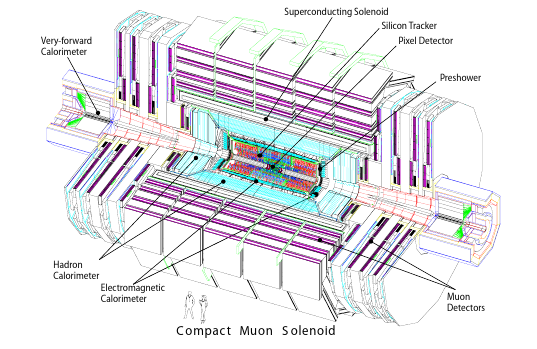
\includegraphics[width=10cm,height=6cm]{Chapter2/cms2.png}
\caption{View of Compact muon solenoid (CMS)}\label{cms}
\end{figure}
	
The resistive plate chamber allows increase the measurement efficiency of the crossing beam at higher luminosities. The RPC are located in the barrel and endcap regions , and have a dedicated triggering detector system that can provide measurements in the range of $|\eta|<1.6$.\\
\pagebreak

RPC are structured in a double gap chambers.
Each gap has a 2 mm thick resistive bakelite separated by a 2mm gass gap that are coated with a conductive graphite layer. They operate a voltage of 9.6 kV . The gas mix used in the RPC consist of 95.2$\%$ Freon
($C_2 H_2 F_4$ ), 4.5$\%$ isobutane ($C_4 H_{10}$), and 0.3$\%$ sulphur hexafluoride (SF$_6$ ). The distribution of the RPC in the barrel and the endcap is similar to DT and CSC ; 4 stations in the barrel and 3 in the endcap.\cite{cms7}


\begin{figure}[!htbp]
	\centering
	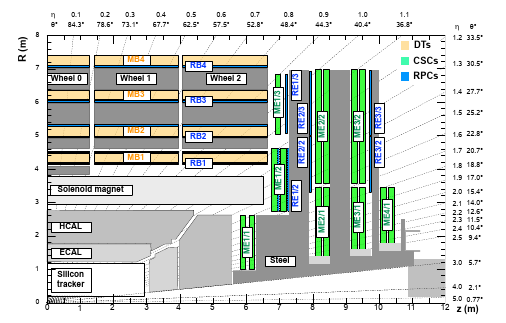
\includegraphics[width=11cm,height=7cm]{Chapter2/csc}
	\caption{Cross section of a quadrant of the CMS with axis parallel to the beam (z axis) horizontally and the radius of the detector in terms of the $\eta$.}
	\label{dt}
\end{figure}

The array of the DT , CSC and RPC are shown in the figure \ref{dt}. The vertical lines represent the endgap and the horizontal the muon barrel. The orange sections are the DTs , where the 4 DTs are labeled MB,CSC marked in green are labeled ME or muon endcap and RPC are the blue lines that are located in the barrel and the endcap. RPC are labeled RB and RE respectively. 
\\

The produced muons are measured in three zones: in the inner tracker, after the coil, and in
the return flux. Measurement the momentum of muons in the muon detector is determined by the muon bending angle at the exit of the 4T coil with the interaction point as the origin of the muon.\cite{cms7}\cite{cms-manual}




\chapter{Statistical Analysis}

\section{Statistical model}
In particle physics experiments one often searches for processes that have been predicted
but not yet seen


\section{Previous results for  \texorpdfstring{${t\bar{t}H+tH}$}  production}
% Uncomment this line, when you have siunitx package loaded.
%The SI Units for dynamic viscosity is \si{\newton\second\per\metre\squared}.
The discovery of a Higgs boson by the CMS and ATLAS experiments in 2012 opened a new field for exploration in the realm of particle physics. It is critical to study the couplings of
this new particle to other elementary particles to test whether it is the Higgs boson as predicted
by the standard model (SM). Of particular interest is the Yukawa coupling of the Higgs boson
to top quarks,$y_t$, as the top quark is widely believed to play a special role in the mechanism
of electroweak symmetry breaking due to its large mass.

Direct searches for tHq production using all relevant Higgs decay modes have previously been
carried out by CMS in the 8 TeV dataset  and in the 2015 13 TeV dataset using the H $\rightarrow$
b$\bar{b}$ channel. In the full 2016 13 TeV dataset, a search for t$\bar{b}$H production in multilepton
final states recently produced first evidence for associated production of top quarks and Higgs
bosons.

\section{Event selection}
The main analysis strategy is to obtain a selection of events compatible with certain characteristics of the signal at pre-selection level.\\
It is required:
\begin{itemize}
\item The events are selected those that contain two leptons ($l^+l^-$)  with the same sign.
\item Transverse moment $p_{t}$ > 25 and 15 GeV, for the muons.
\item A foward jet with $p_t$ > 40 GeV, | $\eta$ | > 2.4
\item One or more b-jets with (| $\eta$ | <2.4)
\end{itemize}



\begin{itemize}
	\item Rare SM: tttt,WWW,WWZ,WZZ,WW,tZq
	\item WZ:WZ,ZZ
\end{itemize}

\section{Boosted decision tree}
BDT Variables 

\begin{itemize}
\item	Trailing lepton $p_{t}$
\item 	Total charge of tight leptons
\item 	min $\Delta$R (lepton pairs)
\item 	$\Delta\phi$ between highest $p_t$ lepton pair
\item 	Number of jets with |$\eta$| < 2.4
\item	Number of non b-tagged jets with |$\eta$| > 1.0
\item	Maximum |$\eta$| for jets
\item	$\Delta\eta$ (most forward light jet, closest lepton)
\item	$\Delta\eta$ (most forward light jet, hardest loosely b-tagged jet)
\item	$\Delta\eta$ (most forward light jet, 2nd hardest loosely b-tagged jet)
\end{itemize}

Common uncertainties for MC :
\begin{itemize}
	\item Muon identificacion 6$\%$
	\item Dimuon Trigger  1$\%$ 
	\item Luminosity measurement: ~2.6$\%$.
\end{itemize}




The likelihood function is the product of Poisson probabilities for all bins
\begin{align}
L(\mu,\theta)=\prod_{j=1}^{N}\frac{(\mu s_j +b_j)^{n_j}}{n_j !}e^{-(\mu s_j+b_j)}
\end{align}

\begin{itemize}
	\item	N=number of bins
	\item	$\mu$=parameter of signal
	\item	s=signal
	\item	b=background
	\item	n=number of events
\end{itemize}


To test a hypothesized value of $\mu$ we consider the profile likelihood ratio
\begin{align}
\lambda(\mu)=\frac{L(\mu,\hat{\hat{\theta}})}{L(\hat{\mu},\hat{\theta})}
\end{align}

	\begin{itemize}
		\item Here $\hat{\hat{\theta}} $ in the numerator denotes the value of $\theta$ that maximizes L for the specified $\mu$,
		it is the conditional maximum-likelihood (ML) estimator of $\hat{\theta}$ (and thus is a function of $\mu$).
		The denominator is the maximized (unconditional) likelihood function, i.e., $\hat{\mu}$ and $\hat{\theta}$ are
		their ML estimators 
		\item The presence of the nuisance parameters broadens the profile likelihood as a
		function of $\mu$ relative to what one would have if their values were fixed. This reflects the loss
		of information about $\mu$ due to the systematic uncertainties
	\end{itemize}

For purposes of establishing an upper limit on the strength parameter $\mu$ , we consider two
closely related test statistics. First, we may define
\begin{align} 
q_{\mu}=  \Big\{    \begin{array}{ll}
                 -2\ln\lambda(\mu) \qquad \hat{\mu} \leq \mu	\\
0  \qquad \qquad \qquad \hat{\mu}< 0 
                \end{array}
\end{align}
 The reason for setting $q_\mu = 0$
for $\hat{\mu}>\mu $ is that when setting an upper limit, one would not regard data with $\hat{\mu}>\mu $ as
representing less compatibility with $\mu$ than the data obtained, and therefore this is not taken
as part of the rejection region of the test. From the definition of the test statistic one sees that
higher values of $q_\mu$ represent greater incompatibility between the data and the hypothesized
value of $\mu$.


To quantify the level of disagreement we compute the P-value
\begin{align}
P_\mu =\int_{t_\mu}^{\infty}f(t_\mu |\mu) dt_\mu
\end{align}
where $t_\mu$  is the value of the statistic $t_\mu$ observed from the data and $f(t\mu |\mu)$ denotes
the PDF (Probability density function) of t$_\mu$ under the assumption of the signal strength $\mu$
\begin{align}
f(t\mu |\mu)=\frac{1}{\sqrt{2\pi}} \frac{1}{\sqrt{t_\mu}}e^\frac{-t_\mu}{2}
\end{align}

\begin{center}
\begin{figure}
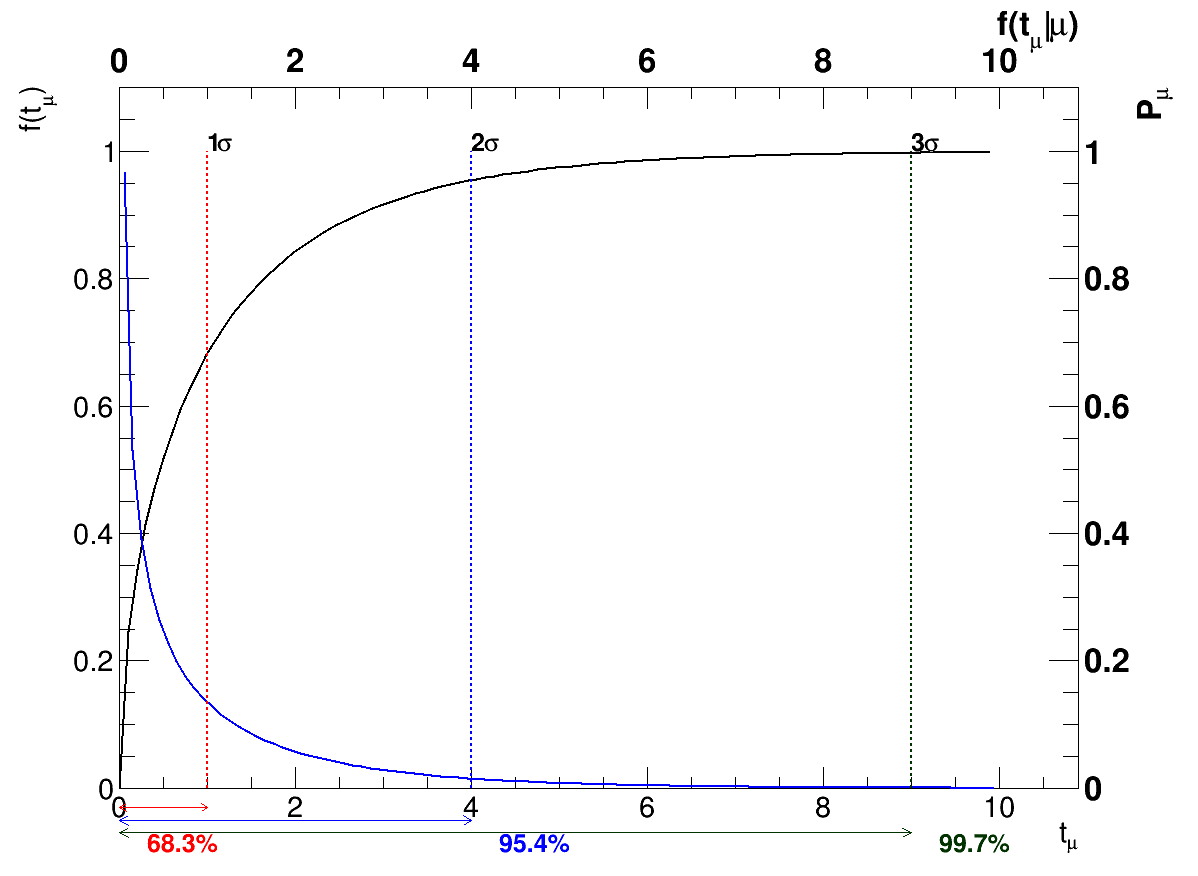
\includegraphics[width=16cm,height=12cm]{Chapter2/nos.png}
\caption{Prueba estad\'istica de $t_\mu$ y P valor para $t_\mu$}
\end{figure}
\end{center}

\begin{center}
\begin{figure}
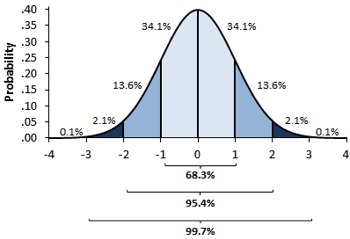
\includegraphics[width=11cm,height=11cm]{Chapter2/normal-curve.jpg}
\caption{Distribuci\'on gaussiana que ilustra los valores de significancia y su probabilidad}
\end{figure}
\end{center}


%Closure:  hay jets en los eventos de tt  (gluon-gluon -> tt + gluon ) que se pasan como muones.  jet -> muon =  fake

%Fakes:   proceso de QCD  que genera muchos  jets (por ejemplo  gluon-gluon -> gluons, quarks)  :    jet -> muons   fakes are estimated data 


\footnote[1]{Due to existence of many uncertainties, it is necessary to sum all the uncertainties. When there is no Correlation, the uncertainties must be summed as the square root of the squares of each uncertainty}

\section{Event selection}
\section{Main Backgrounds}
In the leptonic channels, the main backgrounds are expected to
arise from the production of top quarks
\begin{itemize}
\item In the dominant t$\bar{t}$ mode, where 
same-sign dilepton signatures can occur when a non-prompt lepton from heavy-flavor
decay passes the signal selection, or in associated production with a W/Z or Higgs boson.
\item Processes with single top quarks also contribute, mostly in the associated production with a Z boson (tZ) or when produced with both a W and a Z boson (WZ) 
\item t$\bar{t}$W$^\pm$ and t$\bar{t}$Z (t$\bar{t}$V): Backgrounds are estimated directly from simulated events$\%$ which are corrected for data/MC differences and $\%$ inefficiencies in the same way as signal events. 
\item WZ: Diboson production with leptonic Z decays and additional jet radiation in the final state can
lead to signatures very similar to that of the signal. Due to the larger cross section, the main
contribution arises from WZ production.
\item t$\bar{t}$H: tHq production which decays to same sign deleptons.
\item Rare SM (tZ,VVV,WW,tttt): Due to small event yields, all these process are grouped as one.
\item Non prompt leptons b quark decays and spurious lepton signatures from hadronic jets.
\end{itemize}


\begin{itemize}
\item t$\bar{t}$W$^\pm$ and t$\bar{t}$Z (t$\bar{t}$V): Backgrounds are estimated directly from simulated events$\%$ which are corrected for data/MC differences and inefficiencies in the same way as signal events. 
\item WZ: Diboson production with leptonic Z decays and additional jet radiation in the final state can
lead to signatures very similar to that of the signal. Due to the larger cross section, the main
contribution arises from WZ production.
\item t$\bar{t}$H: tHq production which decays to same sign deleptons.
\item Rare SM (tZ,VVV,WW,tttt): Due to small event yields, all these process are grouped as one.
\item Non prompt leptons b quark decays and spurious lepton signatures from hadronic jets.
\end{itemize}

\begin{table}
\caption{Main backgrounds and their same sign $\mu\mu$ decay process}
\centering
\begin{tabular}{|c|c|c|}
	\hline
	Background & $\sigma$[pb] & Decay process \\
	\hline
t$\bar{t}$H	& 0.2151 & t$\bar{t}$H $\rightarrow$ W$^+$b W$^- \bar{b}$ W$^+$W$^-$ $\rightarrow$ $\mu^+ \nu_\mu$b$\mu^- \bar{\nu_\mu}\bar{b}$ $\mu^+\nu_\mu$ $\mu^-\bar{\nu_\mu}$\\
\hline  
t$\bar{t}$W  &0.2043 &t$\bar{t}$W  $\rightarrow$  W$^+$bW$^- \bar{b}$ $\mu^+\nu_\mu$ $\rightarrow$ $\mu^+ \nu_\mu$b $\mu^- \bar{\nu_\mu} \bar{b}$ $\mu^+ \nu_\mu$\\
\hline
 t$\bar{t}$Z & 0.2529 & t$\bar{t}$Z  $\rightarrow$ W$^+$b  W$^-$$\bar{b} \mu^+ \mu^-$ $\rightarrow$ $\mu^+ \nu_\mu$b $\mu^- \bar{\nu_\mu} \bar{b}\mu^+ \mu^-$  \\
 \hline 
  W$^+$W$^-$  &1.64 & W$^+$W$^-$ $\rightarrow$$\mu^+\nu_\mu$$\mu^-\bar{\nu_\mu}$ \\
    \hline 
  tZq  &0.0758 & tZq$\rightarrow$W$^+$b$\mu^+ \mu^-$ q$\rightarrow$$\mu^+ \nu_\mu$b $\mu^+\mu^-$ q \\
    \hline 
  t$\bar{t}$t$\bar{t}$  & 0.0091&t$\bar{t}$t$\bar{t}$ $\rightarrow$ W$^+$b   W$^- \bar{b}$  W$^+$b  W$^- \bar{b}$   $\rightarrow$ $\mu^+ \nu_\mu$b $\mu^- \bar{\nu_\mu} \bar{b}$ $\mu^+ \nu_\mu$b   $\mu^- \bar{\nu_\mu} \bar{b}$ \\
    \hline 
  W$^+$W$^-$Z  & 0.1651& W$^+$W$^-$Z$\rightarrow$ $\mu^+ \nu_\mu$ $\mu^- \bar{\nu_\mu} \mu^+ \mu^-$\\
    \hline 
 ZZZ  &0.0139 & ZZZ$\rightarrow$ $\mu^+ \mu^-\mu^+ \mu^-l^+ l^-$  \\
    \hline 
  W$^+$ZZ  & 0.0556&W$^+$ZZ$\rightarrow$ $\mu^+ \nu_\mu \mu^+ \mu^- l^+l^-$ \\
  \hline 
 W$^+$Z &4.42965 &W$^+$Z$\rightarrow$ $\mu^+ \nu_\mu \mu^+ \mu^-$ \\
 \hline
ZZ &  1.256 &ZZ$\rightarrow$ $\mu^+ \mu^- \mu^+ \mu^-$ \\
 \hline
\end{tabular}
\end{table}




\begin{tabular}{|l|p{6cm}|l|}
\hline
{Background}& {Sources of systematic uncertainty}&{Total Systematic Uncertainty} \\
\hline
t$\bar{t}$H  & \begin{itemize}
 	\item PDF 4$\%$ 
 	\item QCD scale 5.8$\%$
 	\item Higgs BR  1$\%$ 
 	\end{itemize}
 & 9.36$\%$ \\
 \hline  
 t$\bar{t}$Z&\begin{itemize} 
 			\item PDF 4$\%$ 
 			\item QCD scale 10$\%$ 
 \end{itemize} & 12.36 $\%$ \\
 \hline
 t$\bar{t}$W&{\begin{itemize} { 
 			\item PDF 4$\%$ 
 			\item QCD scale 12$\%$ 
 		}
 \end{itemize}} &14.03 $\%$ \\
 \hline
 {Rares SM} & {\begin{itemize} 
				\item Rare SM 50$\%$ 
	\end{itemize}}&50.36 $\%$ \\
	\hline
	{WZ} & \begin{itemize}
				\item Sample modelling and statistics 50$\%$ 
	\end{itemize} & 50.36$\%$ \\
	\hline 
	{Non prompt leptons} & \begin{itemize} 
				\item Fake rate estimation 50$\%$
				\item Closure 7$\%$ 
	\end{itemize} 		 & 50.48$\%$ \\
	\hline 
\end{tabular}

\section{Systematic uncertainties}
\begin{itemize}
	\item Luminosity measurement: ~2.6$\%$.
	\item Data/MC scale factors for lepton selection (ID, iso) and trigger efficiencies ~5$\%$ per lepton.
	\item Choice of PDF set:
	\begin{itemize}
		\item 3.7$\%$ for tHq
		\item ~4$\%$ for tHW t$\bar{t}$W, t$\bar{t}$Z, t$\bar{t}$H 
		\item Scale uncertainties: 12$\%$, 4 for t$\bar{t}$W, 10$\%$ for t$\bar{t}$Z, +5.8/-9.2$\%$ for t$\bar{t}$H.
	\end{itemize}
	\item Background: WZ, ZZ sample modelling and statistics: ~50$\%$.
	\item Rare SM (tZ,tri-bosons, WWqq, tttt) : 50$\%$
	\item Fake rate estimation:
	The predicted event yield has a normalization uncertainty of ~30-50$\%$ 
\end{itemize}

Detector-simulation related uncertainty
\begin{itemize}
\item Calibrations (electron, jet energy scale)
\item Efficiencies (particle ID, reconstruction)
\item Resolutions (jet energy, muon momentum)
\end{itemize}
Theoretical uncertainties
\begin{itemize}
\item  Factorization/Normalization scale of MC generators
\item Choice of MC generator (ME and/or PS, e.g. Herwig vs Pythia)
\end{itemize}
Monte Carlo Statistical uncertainties
\begin{itemize}\item Statistical uncertainty of simulated samples 
\end{itemize}


\chapter{ tH process}  %Title of the First Chapter




\section{tH production mechanism}
The production of a single top quark in the t channel, where a Higgs boson can be radiated
either from the top quark or from the exchanged W boson in the two dominant leading order
diagrams  provides a unique opportunity to study the relative sign of the coupling.
Any deviation from the standard model coupling structure, where the two diagrams strongly
interfere negatively and thereby suppress the production cross section, can lead to a large enhancement of the event rate.
\begin{center}
\begin{figure}[!htbp]
\centering
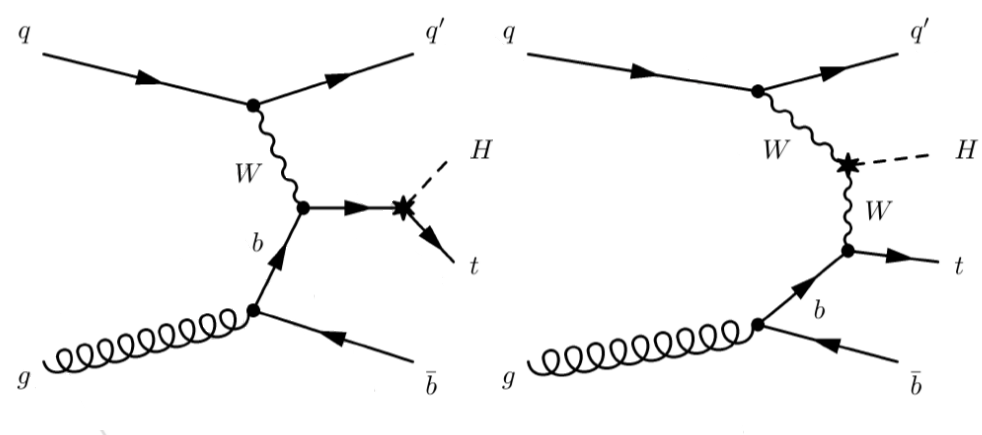
\includegraphics[scale=0.5]{Chapter1/newtHq.png}
\caption{tH mechanism. Higgs radiated from a top quark (left). Higgs radiated from a W boson (right) \protect \cite{bb}} \label{newth}
\end{figure}
\end{center}



\section{Topology of tH}
\begin{center}
\begin{figure}[!htbp]
\centering
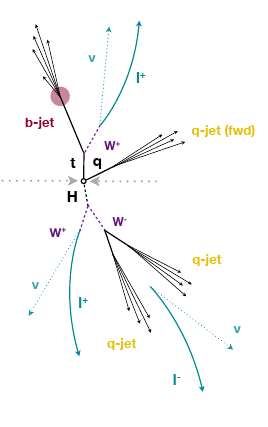
\includegraphics[scale=1.1]{Chapter1/jet.png}\caption{ tH process for $\mu \mu$ final state} \label{jet}
\end{figure}
\end{center}

 For the tH and
ttH processes, the largest contribution comes from Higgs decays to WW (about 75%), followed
by $\tau \tau$ (about 20%) and ZZ (about 5%).

Jets \\
Since quarks and gluons only exist in bound states, we don’t really observe
isolated bare quarks except the top quark, which decays before it has time to form a
bound state. As two quarks are separated, the strong force between them increases
which is equivalent to the potential energy increasing. This energy transforms into
quark-anti-quark pairs. This process of hadronization results in a collimated “jet”
of particles (thesis cms)


\begin{table}
\caption{Table of decay chains for tH.  Expected number of final events assuming 560 produced tH events.l represents $\mu^{\pm},e^- , \tau^\pm$.}
\renewcommand{\arraystretch}{0.55}
\begin{tabular}{|c|c|c|}
\hline
Decay chain & BR & Events\\
\hline 
\small{$tH \rightarrow$ W$^+$bW$^+$W$^-$ $\rightarrow$ $\mu^+$ $\nu_\mu$b$\mu^+\nu_\mu$  $q \bar{q}'$ } &\small{2.096 $\times$10$^{-3}$} &  1.173  \\
\hline
\small{$tH \rightarrow $W$^+$bW$^+$W$^-$ $\rightarrow$ $\mu^+\nu_\mu$b$\mu^+\nu_\mu$ $l^- \bar{\nu_l}$ } &\small{3.37 $\times$ 10$^{-4}$} &0.899 \\
\hline
\small{$tH \rightarrow$ W$^+$b $\tau^+ \tau^-$ $\rightarrow$ $\mu^+ \nu_\mu$ b $ \mu^+ \nu_\mu \bar{\nu_\tau} l^-\bar{\nu_l} \nu_\tau$} &\small{3.637$\times$10$^{-4}$}&0.203 \\
\hline
\small{$tH \rightarrow$ W$^+$bW$^+$W$^-$ $\rightarrow$ $\tau^+ \bar{\nu_\tau}$b $\mu^+ \nu_\mu$  $q\bar{q}$ $\rightarrow$ $\mu^+ \nu_\mu$ $\bar{\nu_\tau}$ $\bar{\nu_\tau}$ b$\mu^+ \nu_\mu$  $q \bar{q}$} &\small{1.890$\times$10$^{-4}$}&0.105  \\
\hline
\small{$tH \rightarrow$ W$^+$b $\tau^+ \tau^-$ $\rightarrow$ $\mu^+$ $\nu_\mu$b $\nu_\tau$ $\mu^+$ $\nu_\mu \bar{\nu_\tau}$} $q \bar{q}$  &
\small{1.681 $\times$10$^{-4}$} & 0.094 \\
\hline
\small{$tH \rightarrow$ W$^+$b W$^+$W$^-$ $\rightarrow$ $\tau^+ \bar{\nu_\tau}$b$ \mu^+ \nu_\mu l^- \bar{\nu_l}$ $\rightarrow$ $\mu^+\nu_\mu$ $ \bar{\nu_\tau} \bar{\nu_\tau}$  b$ \mu^+ \nu_\mu l^- \bar{\nu_l}$} &\small{3.045$\times$10$^{-5}$}& 0.017\\
\hline
\small{$tH \rightarrow$ W$^+$bZZ $\rightarrow$ $q \bar{q}$bZZ $\rightarrow$ $q \bar{q} $ b $\mu^+ \mu^- \mu^+ \mu^-$} & \small{1.966$\times$10$^{-5}$} &0.011\\
\hline 
\small{$tH \rightarrow$ W$^+$b $\tau^+ \tau^-$ $\rightarrow$ $\tau^+ \bar{\nu_\tau}b$ $\mu^+ \nu_\mu \bar{\nu_\tau} $  $q\bar{q}' \nu_\tau$ $\rightarrow$  $\mu^+ \nu_\mu \bar{\nu_\tau}\bar{\nu_\tau} $b $\mu^+ \nu_\mu \bar{\nu_\tau} $  $q\bar{q}' \nu_\tau$ } &\small{1.549 $\times$10$^{-5}$} &  0.008  \\
\hline
\end{tabular}
\end{table}

\end{linenumbers}
